\documentclass[11pt]{article}
\usepackage[margin=1in, top=0.85in, bottom=0.85in]{geometry}
\usepackage{amsmath}
\usepackage{booktabs}
\usepackage{graphicx}
\usepackage{caption}
\usepackage{hyperref}
\usepackage{enumitem}
\usepackage{titlesec}
\usepackage{float}
\usepackage{array}
\usepackage{tabularx}
\usepackage{parskip}
\usepackage[utf8]{inputenc}
\usepackage[T1]{fontenc}
\usepackage{lmodern}

% Section spacing — tighter than default
\titlespacing*{\section}      {0pt}{1.4ex plus 0.5ex minus 0.2ex}{0.6ex plus 0.2ex}
\titlespacing*{\subsection}   {0pt}{1.2ex plus 0.5ex minus 0.2ex}{0.5ex plus 0.2ex}
\titlespacing*{\subsubsection}{0pt}{1.0ex plus 0.4ex minus 0.2ex}{0.4ex plus 0.2ex}

% Paragraph spacing
\setlength{\parskip}{4pt}
\setlength{\parindent}{0pt}

% List spacing
\setlist{nosep, topsep=2pt, itemsep=2pt, parsep=0pt}

\hypersetup{colorlinks=true, linkcolor=blue, citecolor=blue, urlcolor=blue}

% Custom ragged column type (uses standard p-column, no ragged2e needed)
\newcolumntype{L}[1]{>{\raggedright\arraybackslash}p{#1}}

% ── Caption setup ──────────────────────────────────────────────────────────────
\captionsetup{labelsep=period, font=small, skip=4pt}

\title{\vspace{-2em}\textbf{Movie Memory Experiment}\\[0.4em]
{\large Final Report: Descriptive and Inferential Statistics}}
\author{The Standard Deviants}
\date{}

\begin{document}

\maketitle
\vspace{-1em}

% ══════════════════════════════════════════════════════════════════════════════
\section*{1.\quad Introduction}

Our study investigated whether disrupting natural event boundaries during video viewing effect visual recognition memory. Participants watched YouTube Shorts clips under two conditions: \textbf{Natural Boundary (NB)}, where clips ended at a natural scene transition, and \textbf{Abrupt Boundary (AB)}, where clips were cut 1--5 seconds before the boundary. After viewing, participants completed a two-alternative forced-choice (2AFC) recognition test, identifying target frames (seen) from lure frames (unseen). Targets were drawn from either \textbf{before the boundary (BB)} or the \textbf{event middle (EM)} frames, allowing us to test whether any memory impairment is specific to boundary-adjacent frames or due to whole event.

% ══════════════════════════════════════════════════════════════════════════════
\section*{2.\quad Background}

Human memory does not encode all moments equally. According to \textbf{Event Segmentation Theory} (EST; Zacks et al., 2007), the brain continuously builds a working model of the current situation and generates predictions about what will happen next. When incoming information violates these predictions a \textbf{prediction error} is generated, signalling the start of a new event. This triggers a model update that strengthens memory encoding for boundary-adjacent content, while making prior event information temporarily less accessible (Radvansky \& Zacks, 2017). The result is the \textbf{boundary advantage}: recognition memory is better for frames near event boundaries than for frames from the event middle (Swallow, Zacks, \& Abrams, 2009). By artificially cutting a clip before its natural boundary, the AB condition prevents the normal model-update process from completing, which should weaken the boundary-driven encoding boost and reduce memory for the disrupted content.

% ══════════════════════════════════════════════════════════════════════════════
\section*{3.\quad Dataset Description}

A total of \textbf{185 participants} from IIIT Hyderabad community and are randomly assigned to one of two between-subjects conditions. In the \textbf{Natural Boundary (NB)} condition, participants watched video clips that ended at a natural event boundary. In the \textbf{Abrupt Boundary (AB)} condition, clips were cut 1--5 seconds before the natural boundary.

Each participant watched 45 video clips during encoding 40 unique YouTube Shorts and 5 repeated clips serving as \textbf{vigilance checks} (spacebar press on recognition). After encoding, participants completed a 2AFC recognition test for each unique clip, choosing between a \textbf{target} (seen) and a \textbf{lure} frame (unseen). Targets were either \textbf{BB} or \textbf{EM}. After each decision, participants rated confidence on a 1--5 scale. The measured variables are in Table~1.

\begin{table}[H]
\centering
\small
\caption*{Table 1.\; Measured Variables}
\begin{tabularx}{\textwidth}{@{} l L{2.2cm} X @{}}
\toprule
\textbf{Variable} & \textbf{Type} & \textbf{Description} \\
\midrule
Accuracy    & Binary        & Correctly identified target (1) or incorrect (0) \\
RT          & Cont.\ (s)    & Time from stimulus display to key press \\
Confidence  & Ordinal       & Self-rated certainty (1 = low, 5 = high) \\
Frame Type  & Categorical   & BB (near boundary) or EM (event middle) \\
Condition   & Categorical   & NB (natural boundary) or AB (abrupt boundary) \\
Enc.\ Time  & Cont.\ (min)  & Total time spent watching videos during encoding \\
\bottomrule
\end{tabularx}
\end{table}

% ══════════════════════════════════════════════════════════════════════════════
\section*{4.\quad Methods}

\subsection*{4.1\quad Participant Demographics}

A total of \textbf{185 participants} were recorded, of whom \textbf{171} had usable behavioural data files. Of these, \textbf{163} had valid demographic records; the remaining \textbf{22} participants were missing demographic information. For all demographic analyses, these missing values were imputed using the group mean (for age) or group mode (for categorical variables). Both groups remained well-matched on all demographic variables; a breakdown is given in Table~2.

\begin{table}[H]
\centering
\small
\caption*{Table 2.\; Participant Demographics by Condition}
\begin{tabular}{@{} l l c c @{}}
\toprule
\textbf{Variable}   & \textbf{Category} & \textbf{AB} & \textbf{NB} \\
\midrule
\textbf{Age}        & Range (years)     & \multicolumn{2}{c}{19--34} \\
                    & Mean (SD)         & 22.3 (2.3) & 22.3 (2.4) \\
\midrule
\textbf{Gender}     & Male              & 55 & 58 \\
                    & Female            & 27 & 23 \\
\midrule
\textbf{Handedness} & Right-handed      & 79 & 75 \\
                    & Left-handed       &  3 &  6 \\
\midrule
\textbf{Vision}     & Normal            & 44 & 40 \\
                    & Corrected         & 38 & 39 \\
                    & Uncorrected       &  0 &  2 \\
\bottomrule
\end{tabular}
\end{table}

\subsection*{4.2\quad Data Cleaning}

\textbf{Incomplete data.}\; The file for participant sub42 (NB) contained only demographic output with no recognition trial data. Participant sub20 data was unavailable. Both were excluded from all analyses.

\textbf{Excessive encoding time.}\; The five repeated clips account for 5.6 minutes of total encoding time; assuming 25 seconds per repeated-clip recognition, participants spending more than 27.05 minutes in total were deemed inattentive. Four participants exceeded this threshold and were excluded (Table~3).

\begin{table}[H]
\centering
\small
\caption*{Table 3.\; Participants Excluded for Excessive Encoding Time}
\begin{tabular}{@{} c c c @{}}
\toprule
\textbf{Participant} & \textbf{Condition} & \textbf{Enc.\ Time (min)} \\
\midrule
sub32  & AB & 27.33 \\
sub36  & AB & 27.77 \\
sub151 & NB & 27.16 \\
sub161 & NB & 28.00 \\
\bottomrule
\end{tabular}
\end{table}

\textbf{Response time outliers.}\; Trials with RT $< 0.2$ s or RT $> 60$ s were excluded. One outlier was identified: sub28 (AB, Movie~8, RT~$= 71.09$ s).

\textbf{Response time cleaning.} In some of the analysis we used the distributions and applied data cleaning. Trials with response times (RT) greater than $Mean + 4 \times SD$  were removed to minimize the impact of inattentiveness. This resulted in the removal of 54 trials (0.8\% of total data).

\textbf{Condition re-classification.}\; Participant sub157 was labelled AB in the filename, but the video path column confirmed NB stimuli were viewed. Sub157 was re-classified to NB.

\textbf{Missing demographic data.}\; Twenty-two participants who did not fill the demographic form had their data imputed with group means or modes for demographic equivalence testing (H6) and are retained in all analyses.

After all exclusions, the \textbf{final analysed sample comprised 166 participants} (AB: $n = 78$; NB: $n = 88$).

% ─────────────────────────────────────────────────────────────────────────────
\subsection*{4.3\quad Hypotheses}

Based on Event Segmentation Theory, we came up with six hypotheses.

\medskip

% ── H1 ────────────────────────────────────────────────────────────────────────
\begin{table}[H]
\centering\small
\caption*{H1 \;—\; Effect of Condition}
\begin{tabularx}{\textwidth}{@{} l X @{}}
\toprule
\textbf{IV}        & Viewing condition (NB vs.\ AB) --- between subjects \\
\textbf{DV}        & Mean recognition accuracy, mean RT (s) \\
$H_0$              & No difference in accuracy or RT between NB and AB \\
$H_A$              & Participants in the NB condition will show higher overall recognition accuracy and faster response times than participants in the AB condition.\\
\textbf{Direction} & One-tailed \;(NB $>$ AB accuracy;\; NB $<$ AB RT) \\
\textbf{Test}      & Mann-Whitney U test \& trial-level Regression (for RT) \\
\bottomrule
\end{tabularx}
\end{table}

% ── H2 ────────────────────────────────────────────────────────────────────────
\begin{table}[H]
\centering\small
\caption*{H2 \;—\; Effect Larger for BB Frames}
\begin{tabularx}{\textwidth}{@{} l X @{}}
\toprule
\textbf{IV}        & Viewing condition (NB vs.\ AB) --- between subjects \\
\textbf{DV}        & Mean recognition accuracy for BB frames \\
$H_0$              & No difference in BB accuracy between conditions \\
$H_A$              & Recognition accuracy will be greater for before-boundary (BB) frames than for event-middle (EM) frames.Reflecting NB advantage\\
\textbf{Direction} & One-tailed \;(Accuracy : BB > EM) \\
\textbf{Test}      & Independent-samples $t$-test \\
\bottomrule
\end{tabularx}
\end{table}

% ── H3 ────────────────────────────────────────────────────────────────────────
\begin{table}[H]
\centering\small
\caption*{H3 \;—\; No Condition Effect for EM Frames}
\begin{tabularx}{\textwidth}{@{} l X @{}}
\toprule
\textbf{IV}        & Viewing condition (NB vs.\ AB) --- between subjects \\
\textbf{DV}        & Mean recognition accuracy for EM frames \\
$H_0$              & Recognition accuracy for EM frames will not differ significantly between the NB and AB groups. \\
$H_A$              & Significant difference in EM accuracy \\
\textbf{Direction} & Two-tailed \;(EM frames are away from the manipulation point) \\
\textbf{Test}      & Independent-samples $t$-test \\
\bottomrule
\end{tabularx}
\end{table}

% ── H4 ────────────────────────────────────────────────────────────────────────
\begin{table}[H]
\centering\small
\caption*{H4 \;—\; Confidence Calibration}
\begin{tabularx}{\textwidth}{@{} l X @{}}
\toprule
\textbf{IV}        & Trial outcome (correct / incorrect) --- within subjects \\
\textbf{DV}        & Mean confidence rating (1--5 scale) \\
$H_0$              & Confidence equal for correct and incorrect trials within each condition (AB and NB) \\
$H_A$              & Within each condition (AB and NB), confidence ratings will be higher for correctly recognised trials than for incorrectly recognised trials \\
\textbf{Direction} & One-tailed \\
\textbf{Test}      & Shapiro-Wilk (normality) $\rightarrow$ Paired $t$-test (if normal) or Wilcoxon Signed-Rank (if non-normal), applied separately per condition \\
\bottomrule
\end{tabularx}
\end{table}

% ── H5 ────────────────────────────────────────────────────────────────────────
\begin{table}[H]
\centering\small
\caption*{H5 \;—\; Confidence by Frame Type}
\begin{tabularx}{\textwidth}{@{} l X @{}}
\toprule
\textbf{IV}        & Frame type (BB vs.\ EM) --- within subjects \\
\textbf{DV}        & Mean confidence rating (1--5 scale) \\
$H_0$              & Confidence equal for BB and EM trials \\
$H_A$              & Confidence ratings will be higher for BB trials than for EM trials. \\
\textbf{Direction} & One-tailed \\
\textbf{Test}      & Paired-samples $t$-test \\
\bottomrule
\end{tabularx}
\end{table}

% ── H6 ────────────────────────────────────────────────────────────────────────
\begin{table}[H]
\centering\small
\caption*{H6 \;—\; Demographic Balance}
\begin{tabularx}{\textwidth}{@{} l X @{}}
\toprule
\textbf{IV}        & Viewing condition (NB vs.\ AB) --- between subjects \\
\textbf{DV}        & Age; gender; handedness; vision status \\
$H_0$              & The NB and AB groups will not differ significantly on age, gender distribution, handedness distribution, or vision status. \\
$H_A$              & Demographic distributions differ significantly \\
\textbf{Direction} & Two-tailed \\
\textbf{Test}      & Independent $t$-test (age);\; $\chi^2$ test (categorical variables) \\
\bottomrule
\end{tabularx}
\end{table}

\subsection*{4.4\quad Statistical Analysis}

Normality of distributions was verified using the Shapiro-Wilk test before each inferential test. Because the data violated normality for H1 (accuracy and RT), H2 (BB frames), and H3 (EM frames) across both groups, we used the non-parametric \textbf{Mann-Whitney U test} in all these cases. For Hypothesis 1, the participant-level comparison was supplemented by a trial-level OLS Linear Regression for RT to evaluate processing speed in greater detail. For H4, where the NB group's difference scores were non-normal ($W = 0.967, p = .025$), the Wilcoxon Signed-Rank test was substituted for the paired $t$-test. For H6 age, the Mann-Whitney U test was similarly applied. In addition to these participant-level tests, we fitted \textbf{trial-level Regression models} (OLS for RT and H5) to evaluate predictive effects without losing trial-level variability. The significance threshold was $\alpha = 0.05$ throughout.

% ══════════════════════════════════════════════════════════════════════════════
\section*{5.\quad Results}

\subsection*{5.1\quad H1 --- Main Effect of Condition}

\subsubsection*{5.1.1\quad Accuracy}

\textbf{Prediction:} 
We expected that participants in the NB condition would have better recognition accuracy than those in the AB condition.

\textbf{Descriptive Statistics:} 
Participants in the NB group identified targets more accurately (average = 87.4\%, SD = 7.0\%, median = 87.5\%) than participants in the AB group (average = 84.0\%, SD = 8.0\%, median = 85.0\%) showing that NB group performed better overall.

\textbf{Assumption Testing:} 
Shapiro-Wilk test confirmed that accuracy data for both groups was not normally distributed (AB: $W = 0.942, p < .001$; NB: $W = 0.914, p < .001$). So we used  non-parametric test (Mann-Whitney U test) to compare the groups.

\textbf{Inferential Statistics:} 
The Mann-Whitney U test showed that the difference in accuracy between the two groups is statistically significant ($U = 2550.5, p = .0042$). 

\textbf{Conclusion:} 
We reject the null hypothesis ($p < .05$) and accept the alternative hypothesis. Supporting the idea from Event Segmentation Theory that keeping natural event boundaries helps improve visual recognition memory.

\subsubsection*{5.1.2\quad Response Time}

\textbf{Prediction:} 
We expected that participants in the NB condition would respond faster than those in the AB condition. 

\textbf{Data Cleaning:}
To make sure the data is accurate, we removed trials where the response time was very high (greater than $M + 4 \times SD$) as mentioned in 4.2.

\textbf{Descriptive Statistics:} 
Contrary to our prediction the NB group ($M = 5.75$ s, $SD = 1.61$ s, $Mdn = 5.55$ s) was not faster than the AB group ($M = 5.59$ s, $SD = 1.32$ s, $Mdn = 5.36$ s). But in fact the NB participants were slightly slower on average. 

\textbf{Assumption Testing:} 
The Shapiro-Wilk test showed that the response time data was not normally distributed for both groups (AB: $W = 0.942, p = .0015$; NB: $W = 0.965, p = .0183$). So we used the non-parametric Mann-Whitney U test to compare the groups. 

\textbf{Inferential Statistics:} 
The Mann-Whitney U test showed that the difference in response time between the two groups is not statistically significant ($U = 3246.0, p = .548$). We also used a trial-level OLS Linear Regression on all responses which showed that the condition was not a significant predictor of response time ($B = 0.162, p = .081$). 

\textbf{Conclusion:} 
We fail to reject the null hypothesis ($p > .05$). This is important as it shows there is no ``speed-accuracy trade-off.'' Meaning the NB group's higher accuracy was not because they took more time but because their memory was actually better.

\begin{figure}[H]
    \centering
    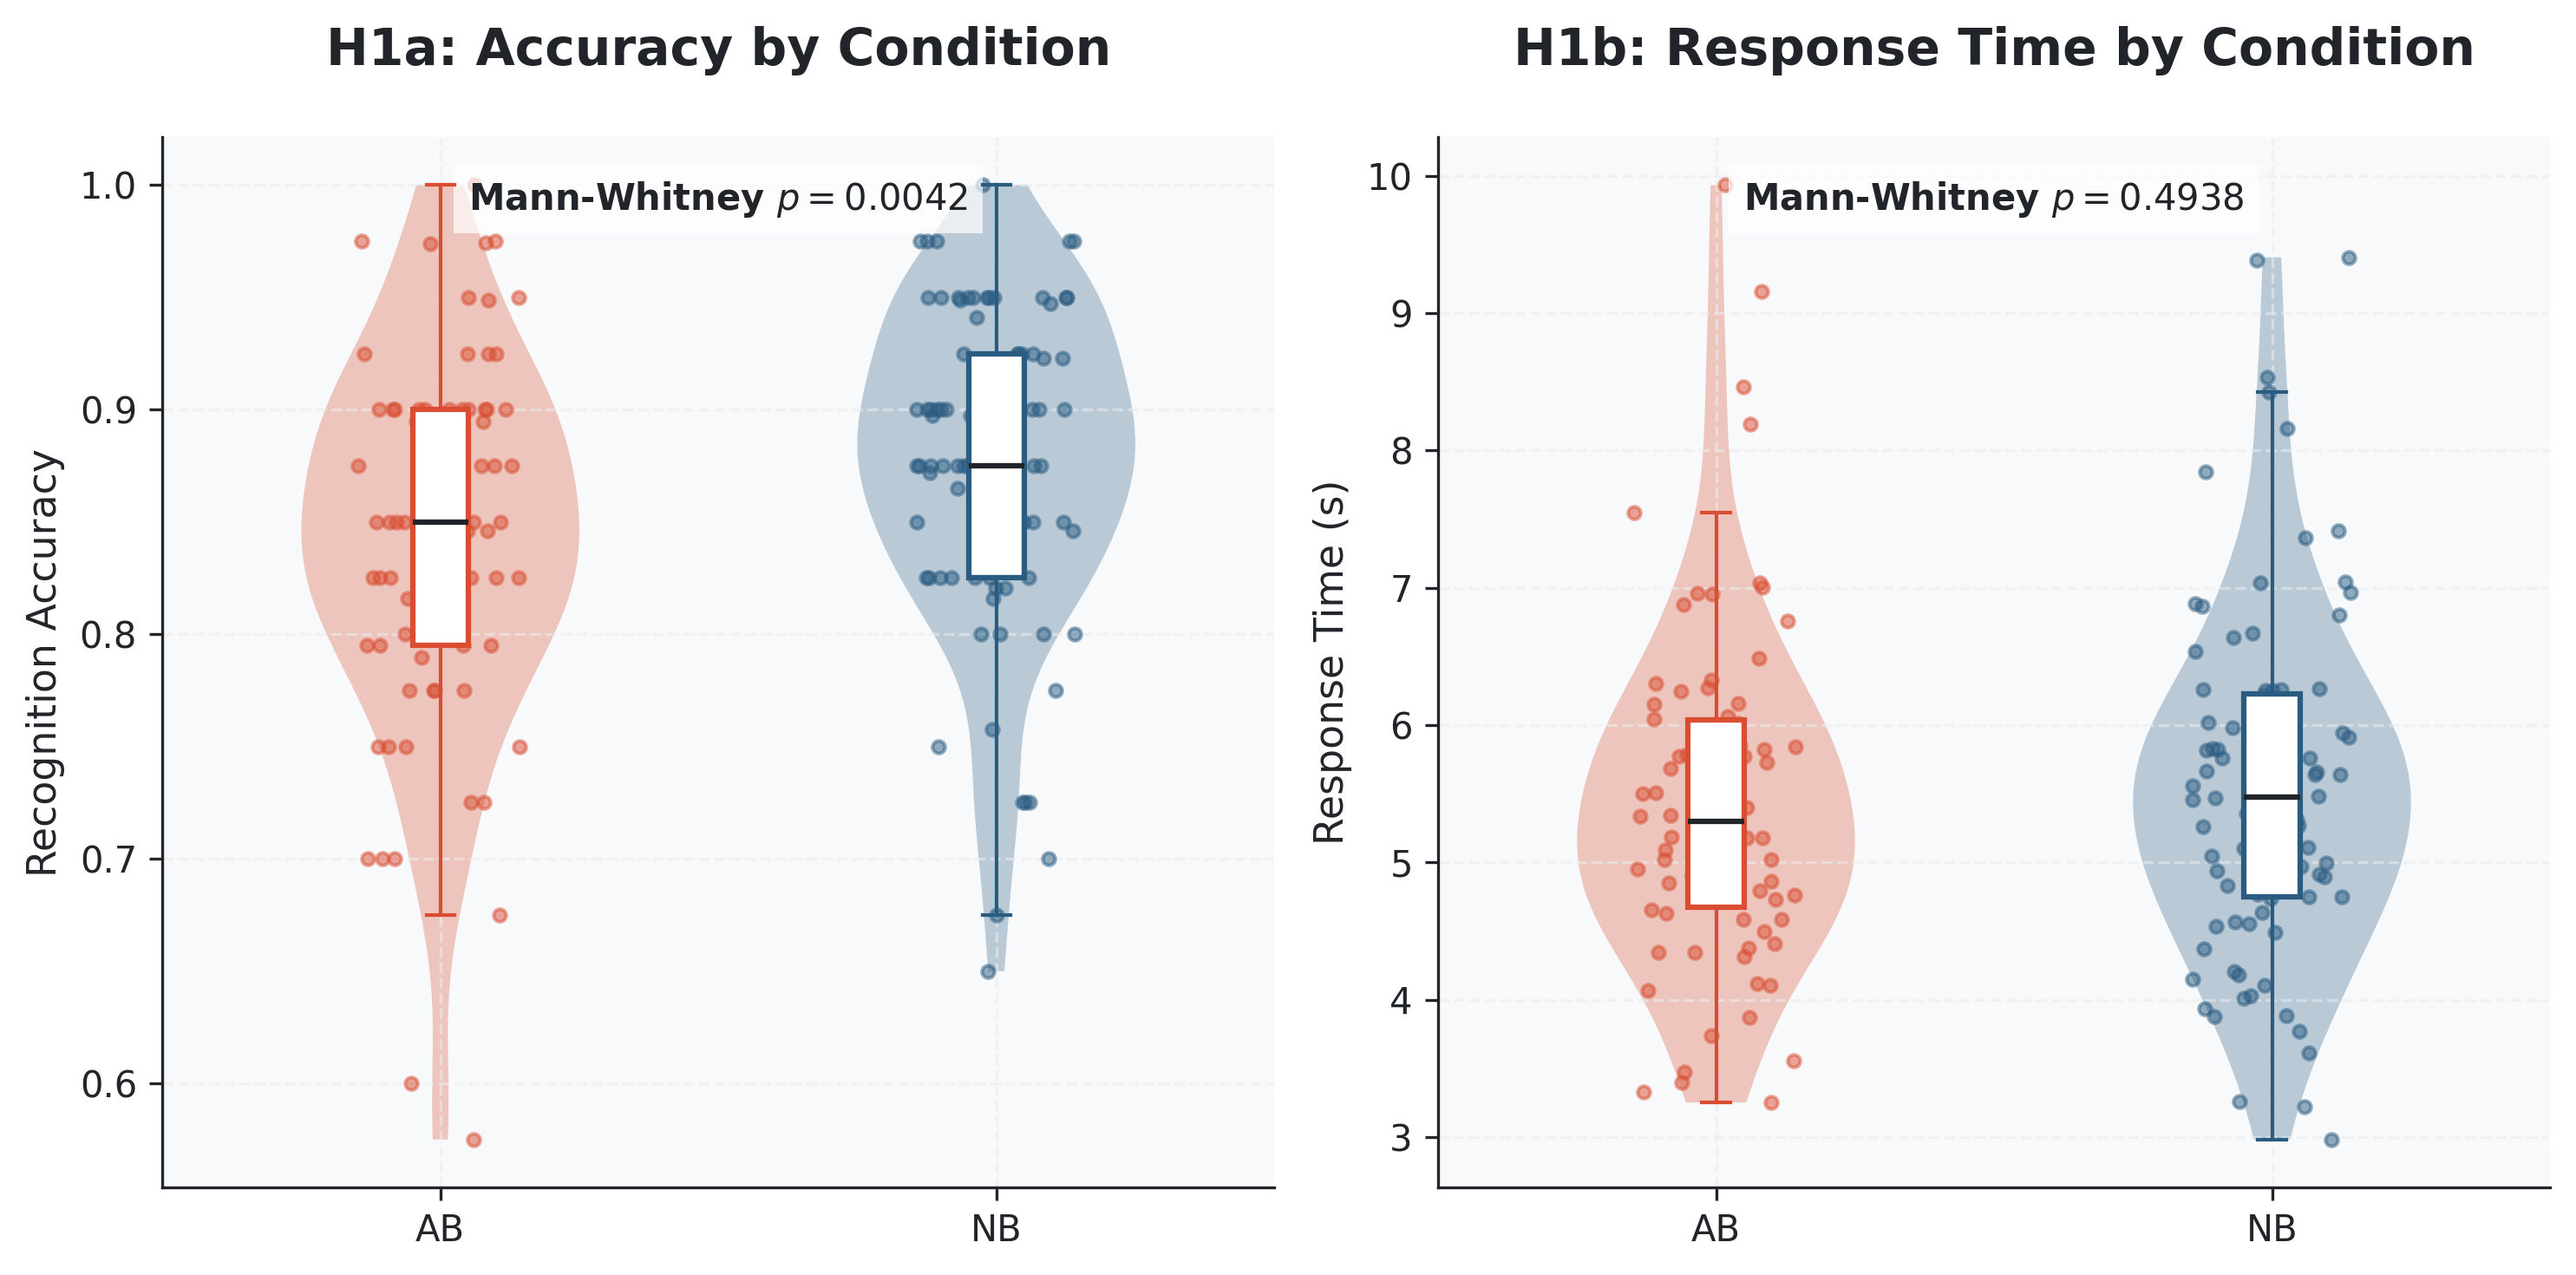
\includegraphics[width=0.82\linewidth]{plots/H1_Accuracy_RT.png}
    \caption*{Figure 5.1 --- H1: Mean recognition accuracy and mean response time by condition (NB vs.\ AB).}
\end{figure}

\subsection*{5.2\quad H2 --- Recognition Accuracy for Pre-Boundary Frames}

\textbf{Prediction:} NB participants would show higher accuracy for before-boundary (BB) frames than AB participants.

\textbf{Rationale:} The boundary advantage predicts that frames just before a natural boundary benefit from heightened perceptual and attentional processing. In the AB condition, the artificial early cut eliminates this encoding boost for BB frames.

\textbf{Normality check.} The Shapiro-Wilk test confirmed that BB-frame accuracy was significantly non-normal in both the AB group ($W = 0.946, p = .002$) and the NB group ($W = 0.925, p < .001$). Consequently, the independent-samples $t$-test was replaced by the \textbf{Mann-Whitney U test}.

\begin{table}[H]
    \centering\small
    \caption*{Table 5.1.\; Mean BB-frame recognition accuracy}
    \begin{tabular}{@{} l c c c c @{}}
        \toprule
        Group & $M$   & $SD$  & $Mdn$ & $n$ \\
        \midrule
        AB    & 0.823 & 0.106 & 0.850 & 77  \\
        NB    & 0.855 & 0.096 & 0.850 & 87  \\
        \bottomrule
    \end{tabular}
\end{table}

NB participants ($M = 0.855$, $Mdn = 0.850$) achieved significantly higher BB-frame accuracy than AB participants ($M = 0.823$, $Mdn = 0.850$): $U = 2705.5$, $p = .032$, rank-biserial $r = 0.192$. This confirms that the natural encoding boost for boundary-adjacent frames is weakened when the boundary is cut short. A trial-level \textbf{Logistic GLM} (accuracy $\sim$ condition, BB trials only) corroborated this finding: being in the NB condition significantly increased the log-odds of a correct response ($B = 0.241$, $z = 2.526$, $p = .012$, $OR = 1.272$; $VIF_{\text{condition}} = 1.000$).

\textbf{H2:} Since $U = 2705.5$ and $p = .032 < \alpha = .05$ (GLM $p = .012$), we \textbf{reject the null hypothesis} and \textbf{support the alternative hypothesis} ($H_A$: NB participants show higher BB-frame accuracy than AB participants). Effect size is small-to-medium (rank-biserial $r = 0.192$).

\subsection*{5.3\quad H3 --- Recognition Accuracy for Event-Middle Frames}

\textbf{Prediction:} EM frame accuracy would not differ significantly between conditions.

\textbf{Rationale:} If the boundary effect only strengthens memory for moments immediately surrounding the boundary, frames from the event middle should be encoded similarly regardless of condition.

\textbf{Normality check.} The Shapiro-Wilk test confirmed non-normality for EM-frame accuracy in both the AB group ($W = 0.923, p < .001$) and the NB group ($W = 0.914, p < .001$). Consequently, the \textbf{Mann-Whitney U test} was used.

\begin{table}[H]
    \centering\small
    \caption*{Table 5.2.\; Mean EM-frame recognition accuracy}
    \begin{tabular}{@{} l c c c c @{}}
        \toprule
        Group & $M$   & $SD$  & $Mdn$ & $n$ \\
        \midrule
        AB    & 0.852 & 0.093 & 0.850 & 77  \\
        NB    & 0.884 & 0.080 & 0.900 & 87  \\
        \bottomrule
    \end{tabular}
\end{table}

Contrary to prediction, NB participants ($M = 0.884$, $Mdn = 0.900$) were also significantly more accurate on EM frames than AB participants ($M = 0.852$, $Mdn = 0.850$): $U = 2648.0$, $p = .019$, rank-biserial $r = 0.209$. A trial-level \textbf{Logistic GLM} (accuracy $\sim$ condition, EM trials only) confirmed the condition effect: being in the NB condition significantly increased accuracy log-odds ($B = 0.280$, $z = 2.701$, $p = .007$, $OR = 1.323$; $VIF_{\text{condition}} = 1.000$). The accuracy drop in the AB group was uniform across both BB and EM frames, suggesting that an abrupt cut impairs memory for the entire clip, not only boundary-adjacent content.

\textbf{H3:} Since $U = 2648.0$ and $p = .019 < \alpha = .05$ (GLM $p = .007$), we \textbf{fail to retain the null hypothesis} ($H_0$: no difference in EM-frame accuracy). Contrary to prediction, the boundary disruption generalises beyond BB frames.

\begin{figure}[H]
    \centering
    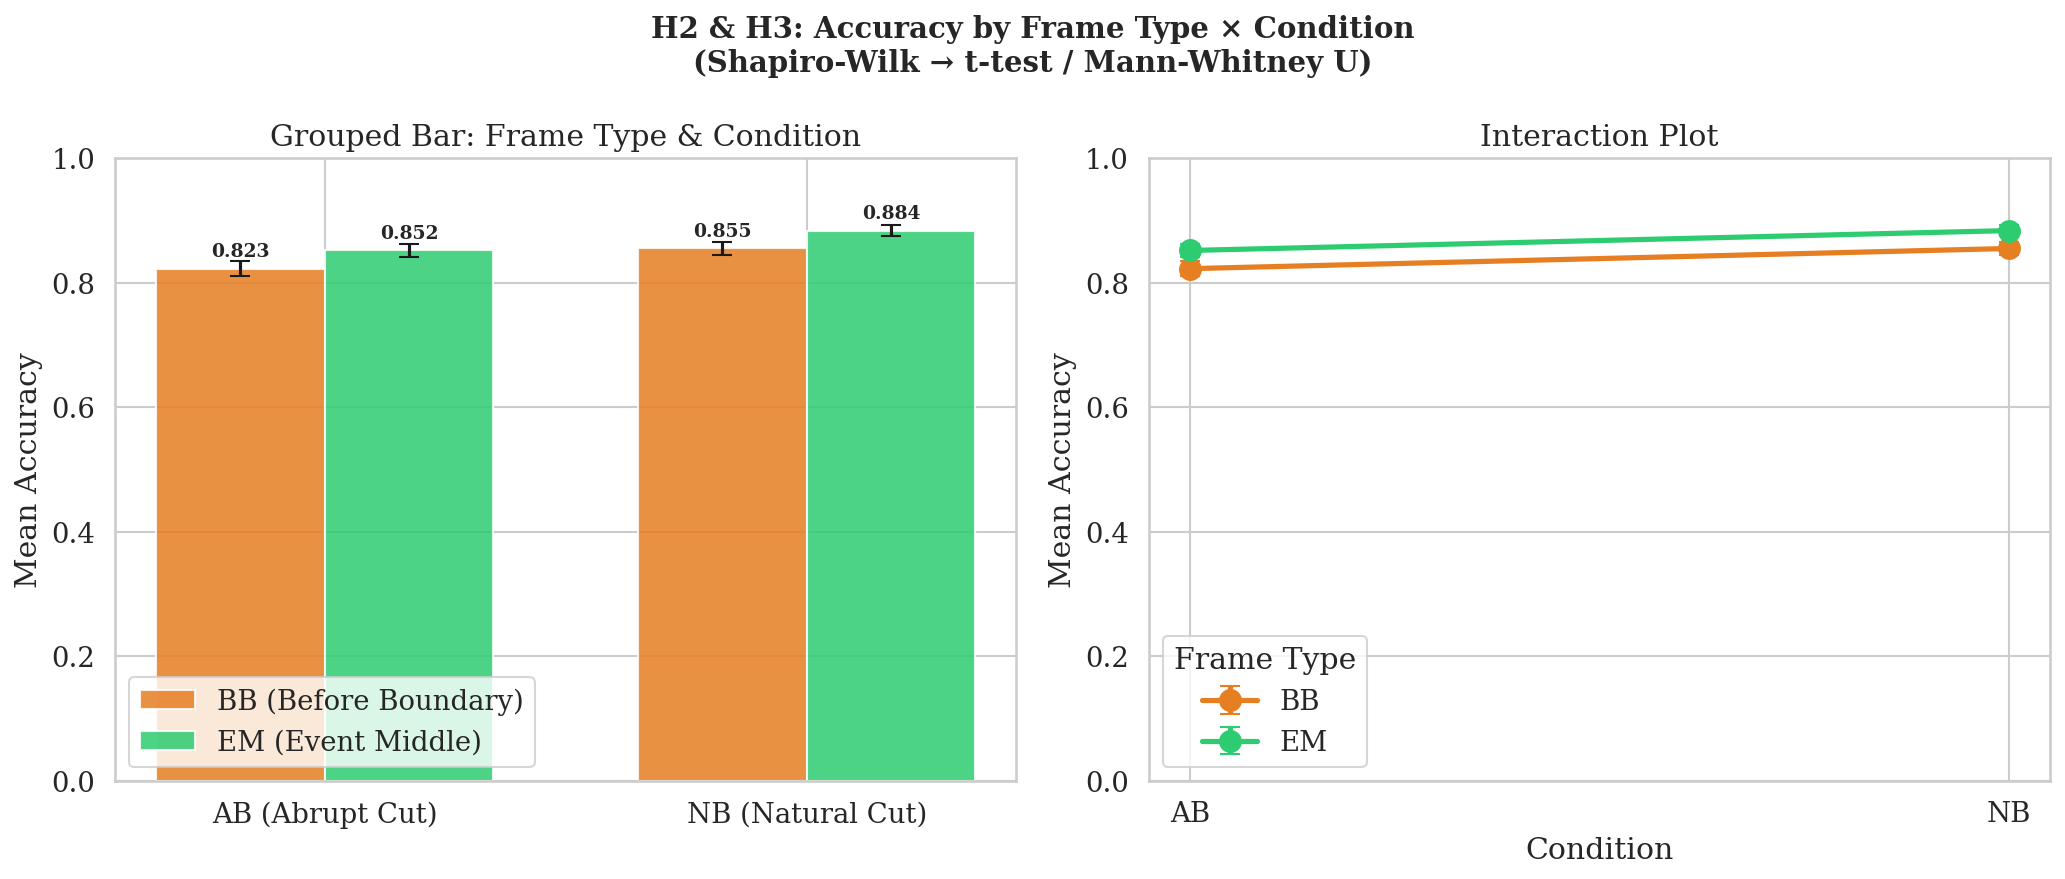
\includegraphics[width=0.82\linewidth]{plots/h2_h3_frame_type.png}
    \caption*{Figure 5.2 --- H2 \& H3: Mean recognition accuracy by frame type (BB, EM) and condition.}
\end{figure}

\subsection*{5.4\quad H4 --- Confidence Calibration}

\textbf{Prediction:} Within each condition (AB and NB), participants would report higher confidence on correct trials than on incorrect trials.

\textbf{Rationale:} If subjective confidence tracks genuine memory signal strength, it should be positively calibrated with accuracy. Analyzing this separately per condition confirms that metacognitive signals are robust regardless of boundary disruption.

One participant who made no errors across the session was excluded from this specific test.

We first evaluated the normality of the differences in confidence ratings using the Shapiro-Wilk test. For the AB group, the distribution was normal ($W = 0.975, p = .134$), leading to a paired $t$-test. For the NB group, the distribution was non-normal ($W = 0.969, p = .033$), requiring the Wilcoxon Signed-Rank test.

\begin{table}[H]
    \centering\small
    \caption*{Table 5.3.\; H4 Results: Confidence Calibration by Condition}
    \begin{tabular}{@{} l c c c c c l @{}}
        \toprule
        Group & Correct $M$ & Incorr. $M$ & Test & Stat & $p$ & Effect Size \\
        \midrule
        AB & 4.201 & 3.362 & $t$-test & $t = 12.562$ & $< .001$ & $d = 1.422$ \\
        NB & 4.311 & 3.356 & Wilcoxon & $W = 50.5$ & $< .001$ & $r = 0.971$ \\
        \bottomrule
    \end{tabular}
\end{table}

In both conditions, participants were significantly more confident when correct than when incorrect ($p < .001$), with the effect consistently in the predicted direction (\textbf{Correct $>$ Incorrect}). Effect sizes were very large ($d = 1.422, r = 0.971$).

\textbf{H4:} Since $p < .001$ for both groups and the direction is correct, we \textbf{reject the null hypothesis} and \textbf{strongly support the alternative hypothesis}.

\begin{figure}[H]
    \centering
    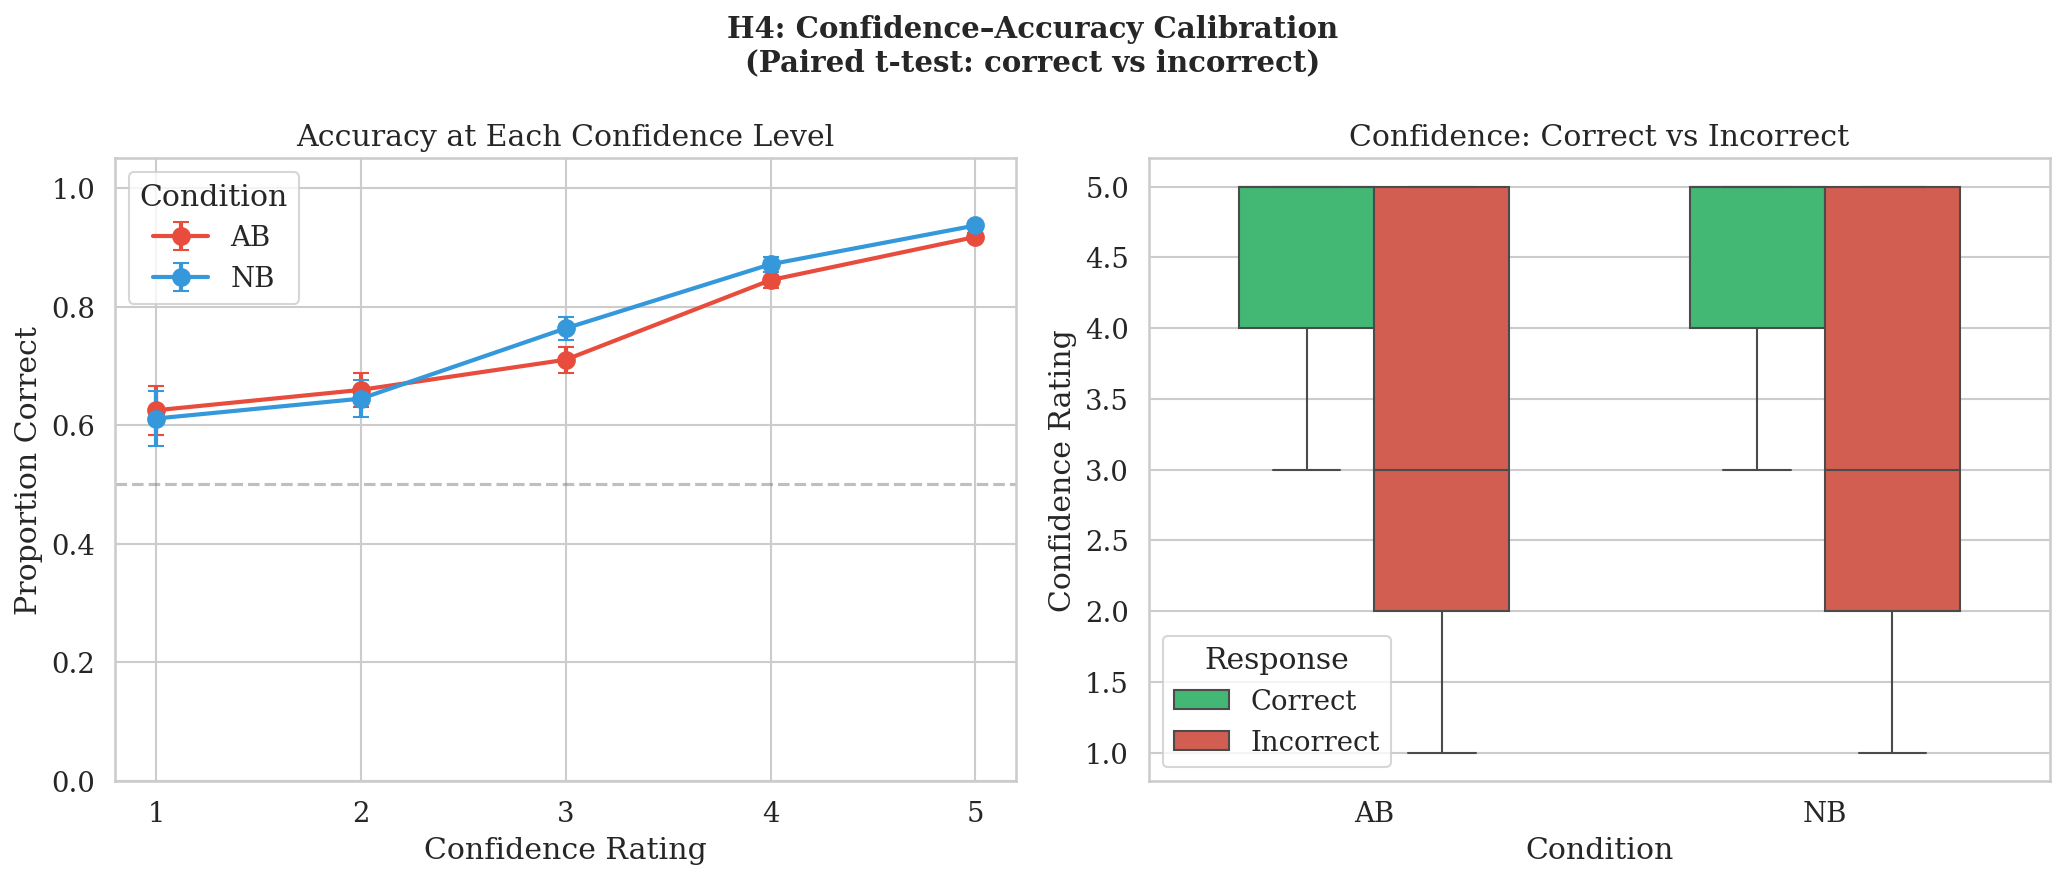
\includegraphics[width=0.82\linewidth]{plots/h4_confidence_accuracy.png}
    \caption*{Figure 5.3 --- H4: Mean confidence ratings for correct vs.\ incorrect trials by condition.}
\end{figure}

\subsection*{5.5\quad H5 --- Confidence by Frame Type}

\textbf{Prediction:} 
We expected that participants would feel more confident for BB frames than EM frames.

\textbf{Data Cleaning:}
Removed trials where the RT was very high greater than $M + 4 \times SD$ as explained in 4.2.

\textbf{Descriptive Statistics:} 
Contrary, participants were not more confident for BB frames. In the AB condition confidence was lower for BB frames ($M = 4.03, SD = 0.52$) compared to EM frames ($M = 4.12, SD = 0.49$). In the NB condition, confidence was mostly same for BB frames ($M = 4.20, SD = 0.55$) and EM frames ($M = 4.22, SD = 0.47$).

\textbf{Assumption Testing:} 
Shapiro-Wilk test showed that the differences between BB and EM frames is a normal distribution for both groups (AB: $W = 0.978, p = .190$; NB: $W = 0.982, p = .265$). So we used paired t-tests to compare them.

\textbf{Inferential Statistics:} 
The paired t-test for the AB group showed a significant difference ($t(77) = -3.004, p = .0036$) but in the opposite direction than expected (EM $>$ BB). For the NB group, the difference was not significant ($p = .4097$).

Trial-level OLS Regression supported the results showing that in the AB condition, confidence for BB frames was significantly lower ($B = -0.091, p = .025$). It also showed that overall confidence was higher in the NB group compared to the AB group ($B = 0.106, p = .008$).

\textbf{Conclusion:} 
Since confidence for BB frames was either lower or not different we reject both the null hypothesis ($H_0$) and the alternative hypothesis ($H_A$). Meaning natural event boundaries do not increase confidence and abrupt cuts actually reduce confidence for moments just before the cut.

\begin{figure}[H]
    \centering
    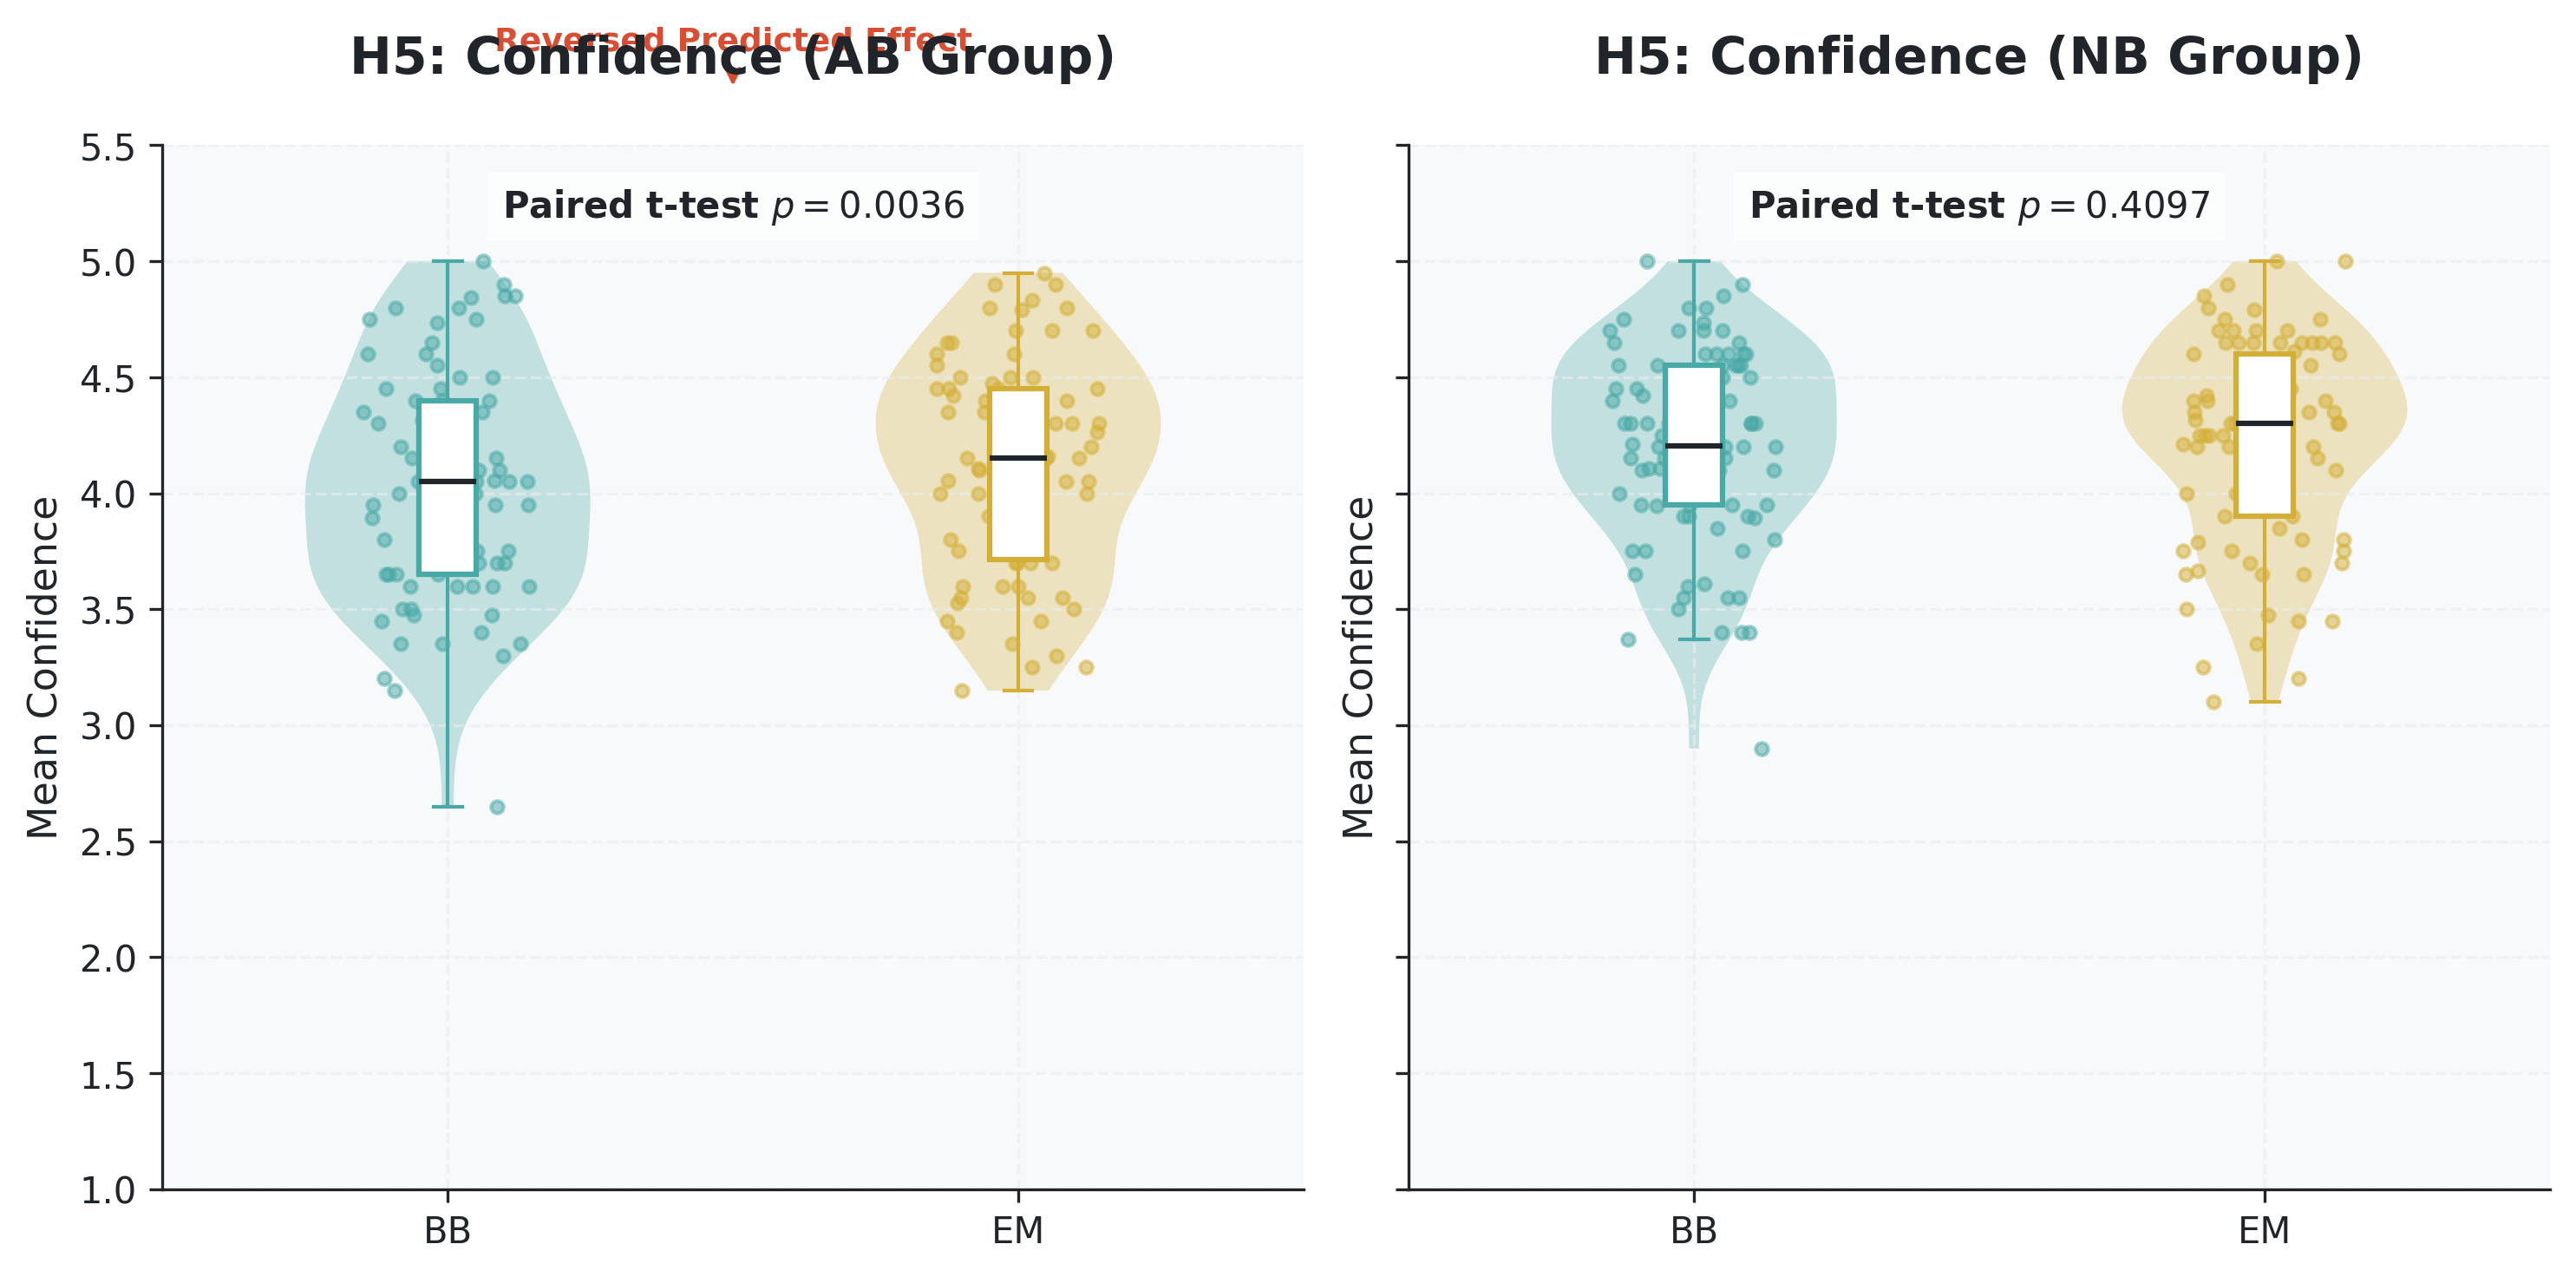
\includegraphics[width=0.82\linewidth]{plots/H5_confidence_frame_type.png}
\caption*{Figure 5.4 --- H5: Mean confidence by frame type (BB vs.\ EM) and condition.}
\end{figure}

\subsection*{5.6\quad H6 --- Demographic Equivalence}

We first evaluated the normality of the age distribution using the Shapiro-Wilk test. Age was found to be significantly non-normal in both AB ($W = 0.855, p < .001$) and NB ($W = 0.929, p < .001$) groups. Consequently, an independent-samples Mann-Whitney U test was used for age. Categorical variables were tested using Chi-square tests of independence.

\begin{table}[H]
    \centering\small
    \caption*{Table 5.5.\; Demographic Balance Checks}
    \begin{tabular}{@{} l c c l c c @{}}
        \toprule
        Variable & AB & NB & Test & Stat & $p$ \\
        \midrule
        Age & Mdn=22.3 & Mdn=22.0 & Mann-Whitney U & $U = 4391.5$ & $.564$ \\
        Gender & 51M, 27F & 55M, 33F & Chi-square & $\chi^2(1) = 0.205$ & $.651$ \\
        Handedness & 71R, 7L & 83R, 5L & Chi-square & $\chi^2(1) = 0.491$ & $.484$ \\
        Vision & 46N, 32C & 45N, 43C & Chi-square & $\chi^2(2) = 2.161$ & $.339$ \\
        \bottomrule
    \end{tabular}
\end{table}

There were no significant differences between groups on any demographic factor (all $p > .05$), confirming that random assignment produced balanced experimental groups.

\textbf{H6:} Since all $p > .05$, we \textbf{fail to reject the null hypothesis} and \textbf{support the alternative hypothesis} (groups are balanced).

\begin{table}[H]
    \centering\small
    \caption*{Table 5.6.\; Participant-level means by condition}
    \begin{tabular}{@{} l c c @{}}
        \toprule
        Variable             & AB ($n = 78$) & NB ($n = 88$) \\
        \midrule
        Accuracy ($M$, $SD$) & 0.84 (0.08)   & 0.87 (0.07)   \\
        RT in s ($M$, $SD$)  & 5.57 (1.42)   & 5.75 (1.63)   \\
        \bottomrule
    \end{tabular}
\end{table}

\begin{figure}[H]
    \centering
    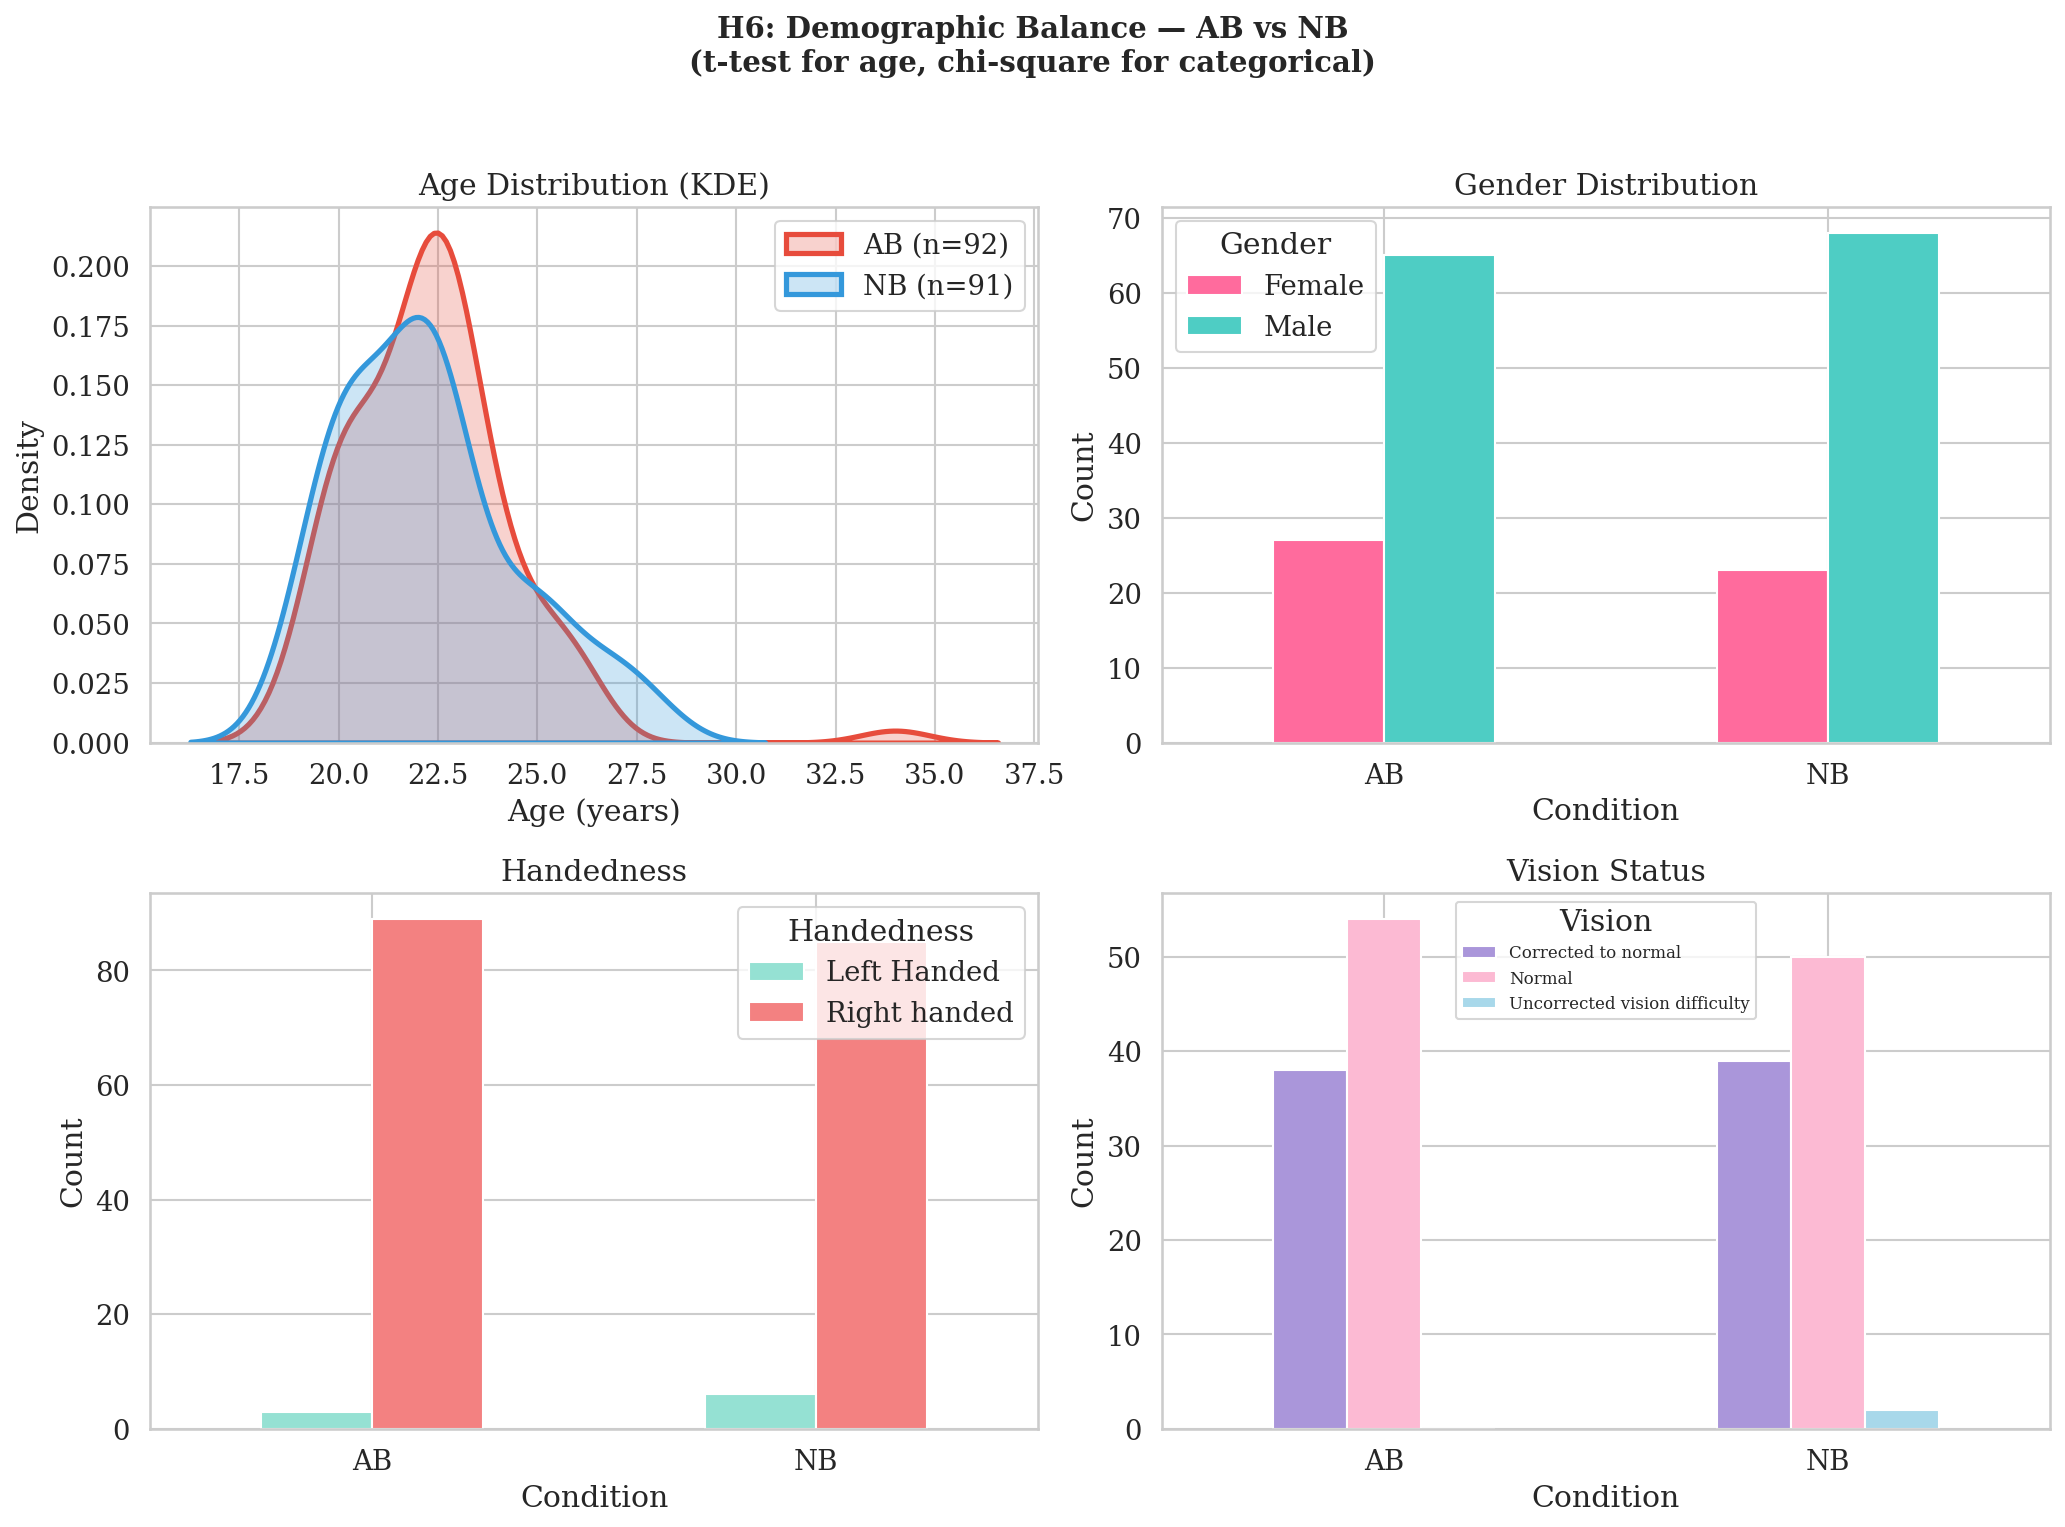
\includegraphics[width=0.82\linewidth]{plots/h6_demographics.png}
    \caption*{Figure 5.5 --- H6: Age and gender distribution by condition.}
\end{figure}

% ─────────────────────────────────────────────
\section*{6.\quad Exploratory Analysis: Predicting Recognition Accuracy}

While our previous tests looked at factors separately, we used a General Linear Model (Logistic Regression) to assess trials simultaneously ($N = 6,640$). This allowed us to test how confidence, experimental condition, and frame type (BB vs.\ EM) jointly predict accuracy. 

\begin{table}[H]
    \centering\small
    \caption*{Table 6.1.\; Logistic Regression Results for Recognition Accuracy}
    \begin{tabular}{@{} l c c c l @{}}
        \toprule
        Predictor & Coef ($B$) & $z$ & $p$ & Odds Ratio \\
        \midrule
        Intercept & $-0.692$ & $-5.99$ & $<.001$ & $0.50$ \\
        Condition (NB) & $0.183$ & $2.51$ & $.012$ & $1.20$ \\
        Frame Type (EM) & $0.208$ & $2.84$ & $.004$ & $1.23$ \\
        Confidence & $0.589$ & $21.21$ & $<.001$ & $1.80$ \\
        \bottomrule
    \end{tabular}
\end{table}

Confidence was the strongest independent predictor of accuracy; for every 1-point increase in subjective confidence, the odds of a correct answer increased by 80.2\% ($OR = 1.80$). Both condition and frame type were also significant predictors, confirming that even when controlling for confidence, the natural-boundary advantage remains. Variance Inflation Factor (VIF) checks confirmed that all predictors were independent ($VIF \approx 1.0$), ensuring the model is stable.

\begin{figure}[H]
    \centering
    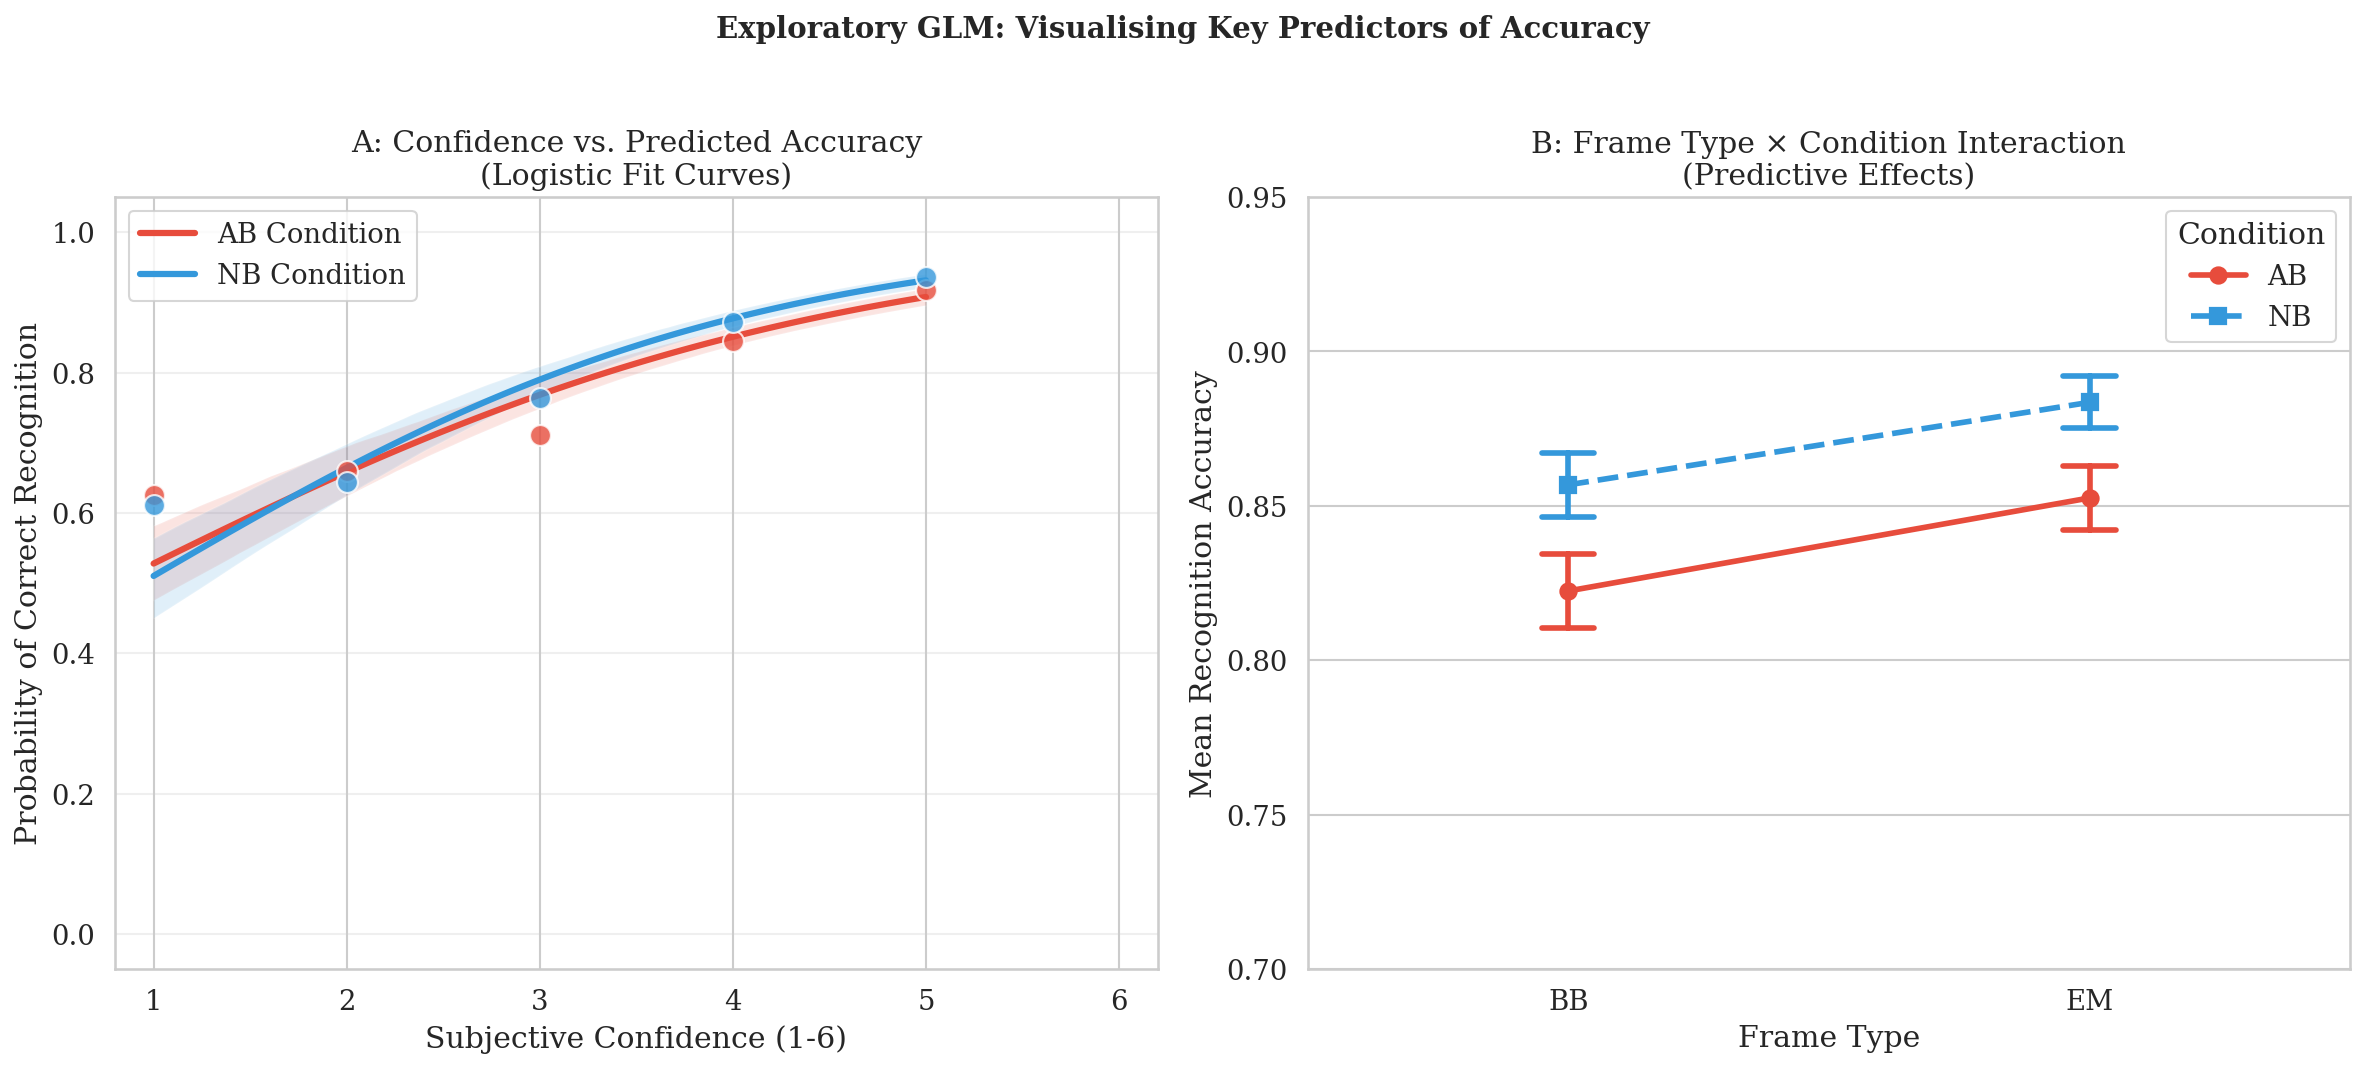
\includegraphics[width=1.0\linewidth]{exploratory_plots/exp_glm_visuals.png}
    \caption*{Figure 6.1: (A) Accuracy predicted by confidence; (B) Effect of video cuts and frame types.}
\end{figure}

% ─────────────────────────────────────────────
\section*{7.\quad Comparison of Results (Report-1 vs. Final Report)}

\subsection*{7.1\quad Recap of Mid-Report (Report-1)}

In our Report-1, we set up the basic steps to analyse our data for evaluating the effect of video cutting methods on memory. For data cleaning, we initially handled missing data by strictly excluding those participants from demographic tests, and we filtered response time outliers by removing trials outside of a $\pm 4 \text{ SD}$ band. Our statistical approach in Report-1 relied heavily on and focused on \textbf{parametric tests} (such as $t$-tests) to evaluate the hypotheses. 

In Report-1, our findings and the associated parametric tests for each hypothesis were as follows:
\begin{itemize}
    \item \textbf{H1 (Effect of Condition):} Evaluated using independent-samples $t$-tests. Supported overall accuracy (NB $>$ AB), but not supported for response time (no speed-accuracy tradeoff).
    \item \textbf{H2 (BB Frame Advantage):} Evaluated using an independent-samples $t$-test. Supported; the Natural Boundary group showed significantly higher accuracy for before-boundary frames.
    \item \textbf{H3 (EM Frame Differences):} Evaluated using an independent-samples $t$-test. Null rejected; the Natural Boundary group unexpectedly also performed better on EM frames.
    \item \textbf{H4 (Confidence Calibration):} Evaluated using a paired-samples $t$-test. Supported; confidence ratings were significantly higher for correct trials than for incorrect trials.
    \item \textbf{H5 (Confidence by Frame Type):} Evaluated using a paired-samples $t$-test. Rejected; confidence was not higher for BB frames, and was paradoxically lower in the AB group.
    \item \textbf{H6 (Demographic Equivalence):} Evaluated using an independent-samples $t$-test (for age) and Chi-square tests. Supported; experimental groups were found to be perfectly balanced across demographics.
\end{itemize}

\subsection*{7.2\quad Methodological Improvements and Validation}

This final report improves how we analysed the data in a few key ways: we shifted heavily to robust \textbf{non-parametric tests} after stricter assumption checking, refined our RT outlier filter to only remove excessively slow trials ($> M + 4 \text{ SD}$), systematically imputed missing demographic data instead of ignoring it, and added a multi-factor Exploratory Analysis.

Despite these robust methodological shifts, \textbf{the final conclusions for all six hypotheses remained identical between Report-1 and this Final Report}. 

\begin{itemize}
    \item \textbf{H1:} Still accepted for Accuracy and rejected for RT. Modifying the data cleaning filter shifted the RT test statistics slightly (e.g., $U$ shifted from $3220.0$ to $3246.0$), but the finding of no significant RT difference remained perfectly stable.
    \item \textbf{H2, H4, \& H6:} Still strongly accepted. Imputing the missing demographic data in this report yielded the exact same equivalence (balanced) result for H6.
    \item \textbf{H3 \& H5:} Still rejected/not supported. This final report confirms the exact same unexpected boundary generalisation trends initially observed in the mid-report.
\end{itemize}



% ─────────────────────────────────────────────
\section*{8.\quad Summary of Findings}

\begin{itemize}
    \item \textbf{Hypothesis 1 (Effect of Condition):} NB participants were significantly more accurate than AB participants ($U=2550.5, p=.0042$), while no significant difference was found in response time ($p=.548$) confirming that preserving natural boundaries improves memory without speed-accuracy trade-off.
    \item \textbf{BB frames (H2):} Shapiro-Wilk confirmed non-normality in both groups; Mann-Whitney U ($U = 2705.5$, $p = .032$, rank-biserial $r = 0.192$) showed NB participants were significantly more accurate on BB frames. Trial-level GLM corroborated: $OR = 1.272$, $p = .012$. The boundary advantage for encoding-adjacent frames is real.
    \item \textbf{EM frames (H3):} Contrary to prediction, EM accuracy also differed significantly ($U = 2648.0$, $p = .019$, $r = 0.209$; GLM: $OR = 1.323$, $p = .007$). The boundary disruption impairs memory for the entire clip, not only boundary-adjacent frames.
    \item \textbf{Confidence (H4):} Strongest result - participants were substantially more confident when correct than incorrect (AB: $d = 1.42$; NB: $r = 0.97$), showing stable metacognitive sensitivity.
    \item \textbf{Confidence by frame type (H5):} The AB group showed \textit{lower} confidence for BB than EM frames --- the opposite of the prediction. No effect in the NB group.
    \item \textbf{Demographics (H6):} Both groups were perfectly matched on all demographic factors (age, gender, handedness, and vision). No sample imbalances were found.
    \item \textbf{Exploratory Analysis (GLM):} Using a multi-factor model with $VIF \approx 1.0$, we found that confidence, condition, and frame type are all independent, significant drivers of recognition accuracy. Confidence is the most powerful predictor, yielding an 80.2\% increase in the odds of accuracy per point.
\end{itemize}


\section*{9\quad References}
{\small\setlength{\parindent}{-2em}\setlength{\leftskip}{2em}\setlength{\parskip}{2pt}

Cutting, J. E., Brunick, K. L., \& Candan, A. (2012). Perceiving event boundaries in motion pictures. \textit{Psychology of Aesthetics, Creativity, and the Arts}, \textit{6}(4), 323--330.

Radvansky, G. A., \& Zacks, J. M. (2017). Event cognition. \textit{Psychological Science in the Public Interest}, \textit{18}(1), 1--57.

Swallow, K. M., Zacks, J. M., \& Abrams, R. A. (2009). Event boundaries in perception affect memory encoding and updating. \textit{Journal of Experimental Psychology: General}, \textit{138}(2), 223--244.

Zacks, J. M., Speer, N. K., Swallow, K. M., Braver, T. S., \& Reynolds, J. R. (2007). Event perception: A mind-brain perspective. \textit{Psychological Bulletin}, \textit{133}(2), 273--293.

}

% ══════════════════════════════════════════════════════════════════════════════
\section*{10.\quad Contributions}

\begin{itemize}
  \item \textbf{Akash} --- Data cleaning, Analysis for H1 and H5, report writing.
  \item \textbf{Varun} --- Analysis for H4 and H6, Exploratory Analysis, report writing
  \item \textbf{Nikhilesh} --- Analysis for H2 and H3, report writing.
\end{itemize}

\medskip
\noindent\textbf{Code Repository.}\quad \url{https://github.com/Varun2345/BRSM-Project}

\end{document}